Certainly! Below is an example of how you might create a TikZ LaTeX diagram that represents the polysemous meanings of a word \( w \) in a semantic tree graph. For this example, let's use the word "mouse" as the root node and generate a graph similar to what you described.

```latex
\documentclass{article}
\usepackage{tikz}

\begin::document

\begin{figure}[h]
    \centering
    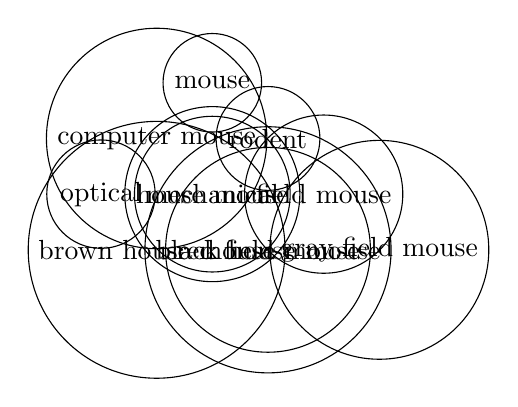
\begin{tikzpicture}[level distance=1.5cm,
                        level 1/.style={sibling distance=3cm},
                        level 2/.style={sibling distance=2cm}]
        % Root Node
        \node[draw,circle] (mouse) {mouse};

        % Level 1: Direct Meanings
        \node[draw,circle] (computerMouse) [below left of=mouse] {computer mouse};
        \node[draw,circle] (rodent) [below right of=mouse] {rodent};

        % Level 2: Sub-Meanings of Computer Mouse
        \node[draw,circle] (optical) [below left of=computerMouse] {optical};
        \node[draw,circle] (mechanical) [below right of=computerMouse] {mechanical};

        % Level 2: Sub-Meanings of Rodent
        \node[draw,circle] (houseMouse) [below left of=rodent] {house mouse};
        \node[draw,circle] (fieldMouse) [below right of=rodent] {field mouse};

        % Level 3: Sub-Meanings of House Mouse
        \node[draw,circle] (brownHouseMouse) [below left of=houseMouse] {brown house mouse};
        \node[draw,circle] (blackHouseMouse) [below right of=houseMouse] {black house mouse};

        % Level 3: Sub-Meanings of Field Mouse
        \node[draw,circle] (redFieldMouse) [below left of=fieldMouse] {red field mouse};
        \node[draw,circle] (grayFieldMouse) [below right of=fieldMouse] {gray field mouse};
    \end{tikzpicture}
    \caption{Graph representation of 'mouse' as the root node, generated by applying our approach to the English Wikipedia corpus.}
    \